\documentclass[english]{article}
\usepackage{hyperref}
\usepackage{amsmath}
\usepackage{graphicx}


\title{ESE 650 Learning in Robotics, Spring 2016 \\ Project 2: Orientation Estimation with Kalman Filters\\
Due: Thursday, Feb 11st \\ Yiren Lu}
\date{}

\newcommand{\mb}{\mathbf }

\begin{document}
\maketitle
\vspace{-30pt}

\section*{Introduction}

For ESE 650 learning in robotics second project, we are provided raw data of the IMU's accelerometer's and gyroscope's data as well as their time stamps to estimate the 3D orientation of the device. And then, use the orientation information to generate a real-time panoramic image from camera. \\
In this project, I firstly converted the raw data from IMU into physical units, and than inferred device orientation in terms of rotation matrices separately from accelerometer and gyroscope. In order to gain robust performance, I implemented an unscented kalman filter (UKF) to combine the accelerometer and gyroscope data. The predicted results were compared with ground truth data from Vicon. Finally, using obtained orientation information, I projected recorded images onto a 3-D cylinder to generate panoramic images. \\




\section {Data Preprocessing}
\subsection {Accelerometer} 
To convert the raw accelerometer data into physical units, the equation is as follows:
\begin{align}
scale\_factor = Vref/(1023 * sensitivity) \\
value = (raw - bias) * scale\_factor 
\end{align}
From the document of ADXL335, we know that $Vref = 3.3v$, $sensitivity = 330 mV/g$,  for the bias, I just simply took the mean of first 100 samples, which are typically stable. And then, correct the z-axis bias of the gravity by substract the z-axis bias of
\begin{equation}
1/ (Vref / 1023 / sensitivity) 
\end{equation}

\subsection {Gyroscope} 
Converting physical values from gyroscope: \\
\begin{align}
value = 3300/1023 * PI/180 / sensitivity 
\end{align}

\section {Rotation Mathematics} 
Rotation group SO(3) has three degrees of freedom. The orientation of the camera is usually be represented in Euler Angles as \emph{roll, pitch} and \emph{yaw}. Detailed explanation and equations that transform between them to be found at \cite{Rotations} and \cite{3dtrans}. In addition, \emph{Quaternions} extend the complex number systems with the properties:
\begin{align}
q = a1 + bi + cj + dk \\
ijk = i^2 = j^2 = k^2 = -1 \\
i = jk \\
k = ij \\
j = ik 
\end{align}
where, $q$ is a quaternion, $a, b, c, d$ are real numbers, $i,j,k$ are imaginary basis elements of the quaternions.\\
Unit Quaternion is a 4 dimensional sphere that could be used to represent orientation and rotation. I used Quaternions to represent the orientation and rotation tranformation heavily in this project.

\subsection {Roll and Pitch from accelerometer}
From accelerometer, we can estimate the gravity direction, from which, we could obtain roll and pitch angles as follows:
\begin{align}
Roll = -arctan(Acc_y/ \sqrt{Acc_x^2 + Acc_z^2}) \\
Pitch = arctan(Acc_x/ \sqrt{Acc_y^2 + Acc_z^2})
\end{align}

\subsection {Orientation Estimation by Gyroscope}
From gyroscope, we can get the angular velocity. By accumulating the angular velocity, we can estimate the orientation of the device at a certain time. The rotation transformation could be representation in \emph{Quaternions}. We can formulate the quaternion rotation given angular velocity $\vec\omega$ and time duration $\Delta t$ from IMU as follows:
\begin{align}
\vec{e} = &\frac{\vec\omega}{||\vec\omega||}\\
\Delta \alpha =& ||\vec\omega||*\Delta t\\
\Delta  q =& [cos(\Delta\alpha/2) \text{  } \vec e sin(\Delta\alpha/2)]\\
q_k+1 = & q_k \Delta q 
\end{align}
Where, $q_k$ is the previous rotation state, $\Delta q$ is the rotation quaternion, and $q_{k+1}$ is the transformed state. We can compute the corresponding rotation matices from $q_k$.

\section {Approaches}
\subsection {Naive Accelerometer and Gyro's Estimation}
From the previous section we know that we could directly compute the orientation matrices from Accelerometer and Gyro data. 
In Figure \ref{fig:naive_4} and \ref{fig:naive_8}, we can see that the acceleroemters' estimation for roll and pitch is generelly well. Gyro instead could catch yaw angle. However, driftings are seemed in gyro's predictions. 


\begin{figure}
\centering
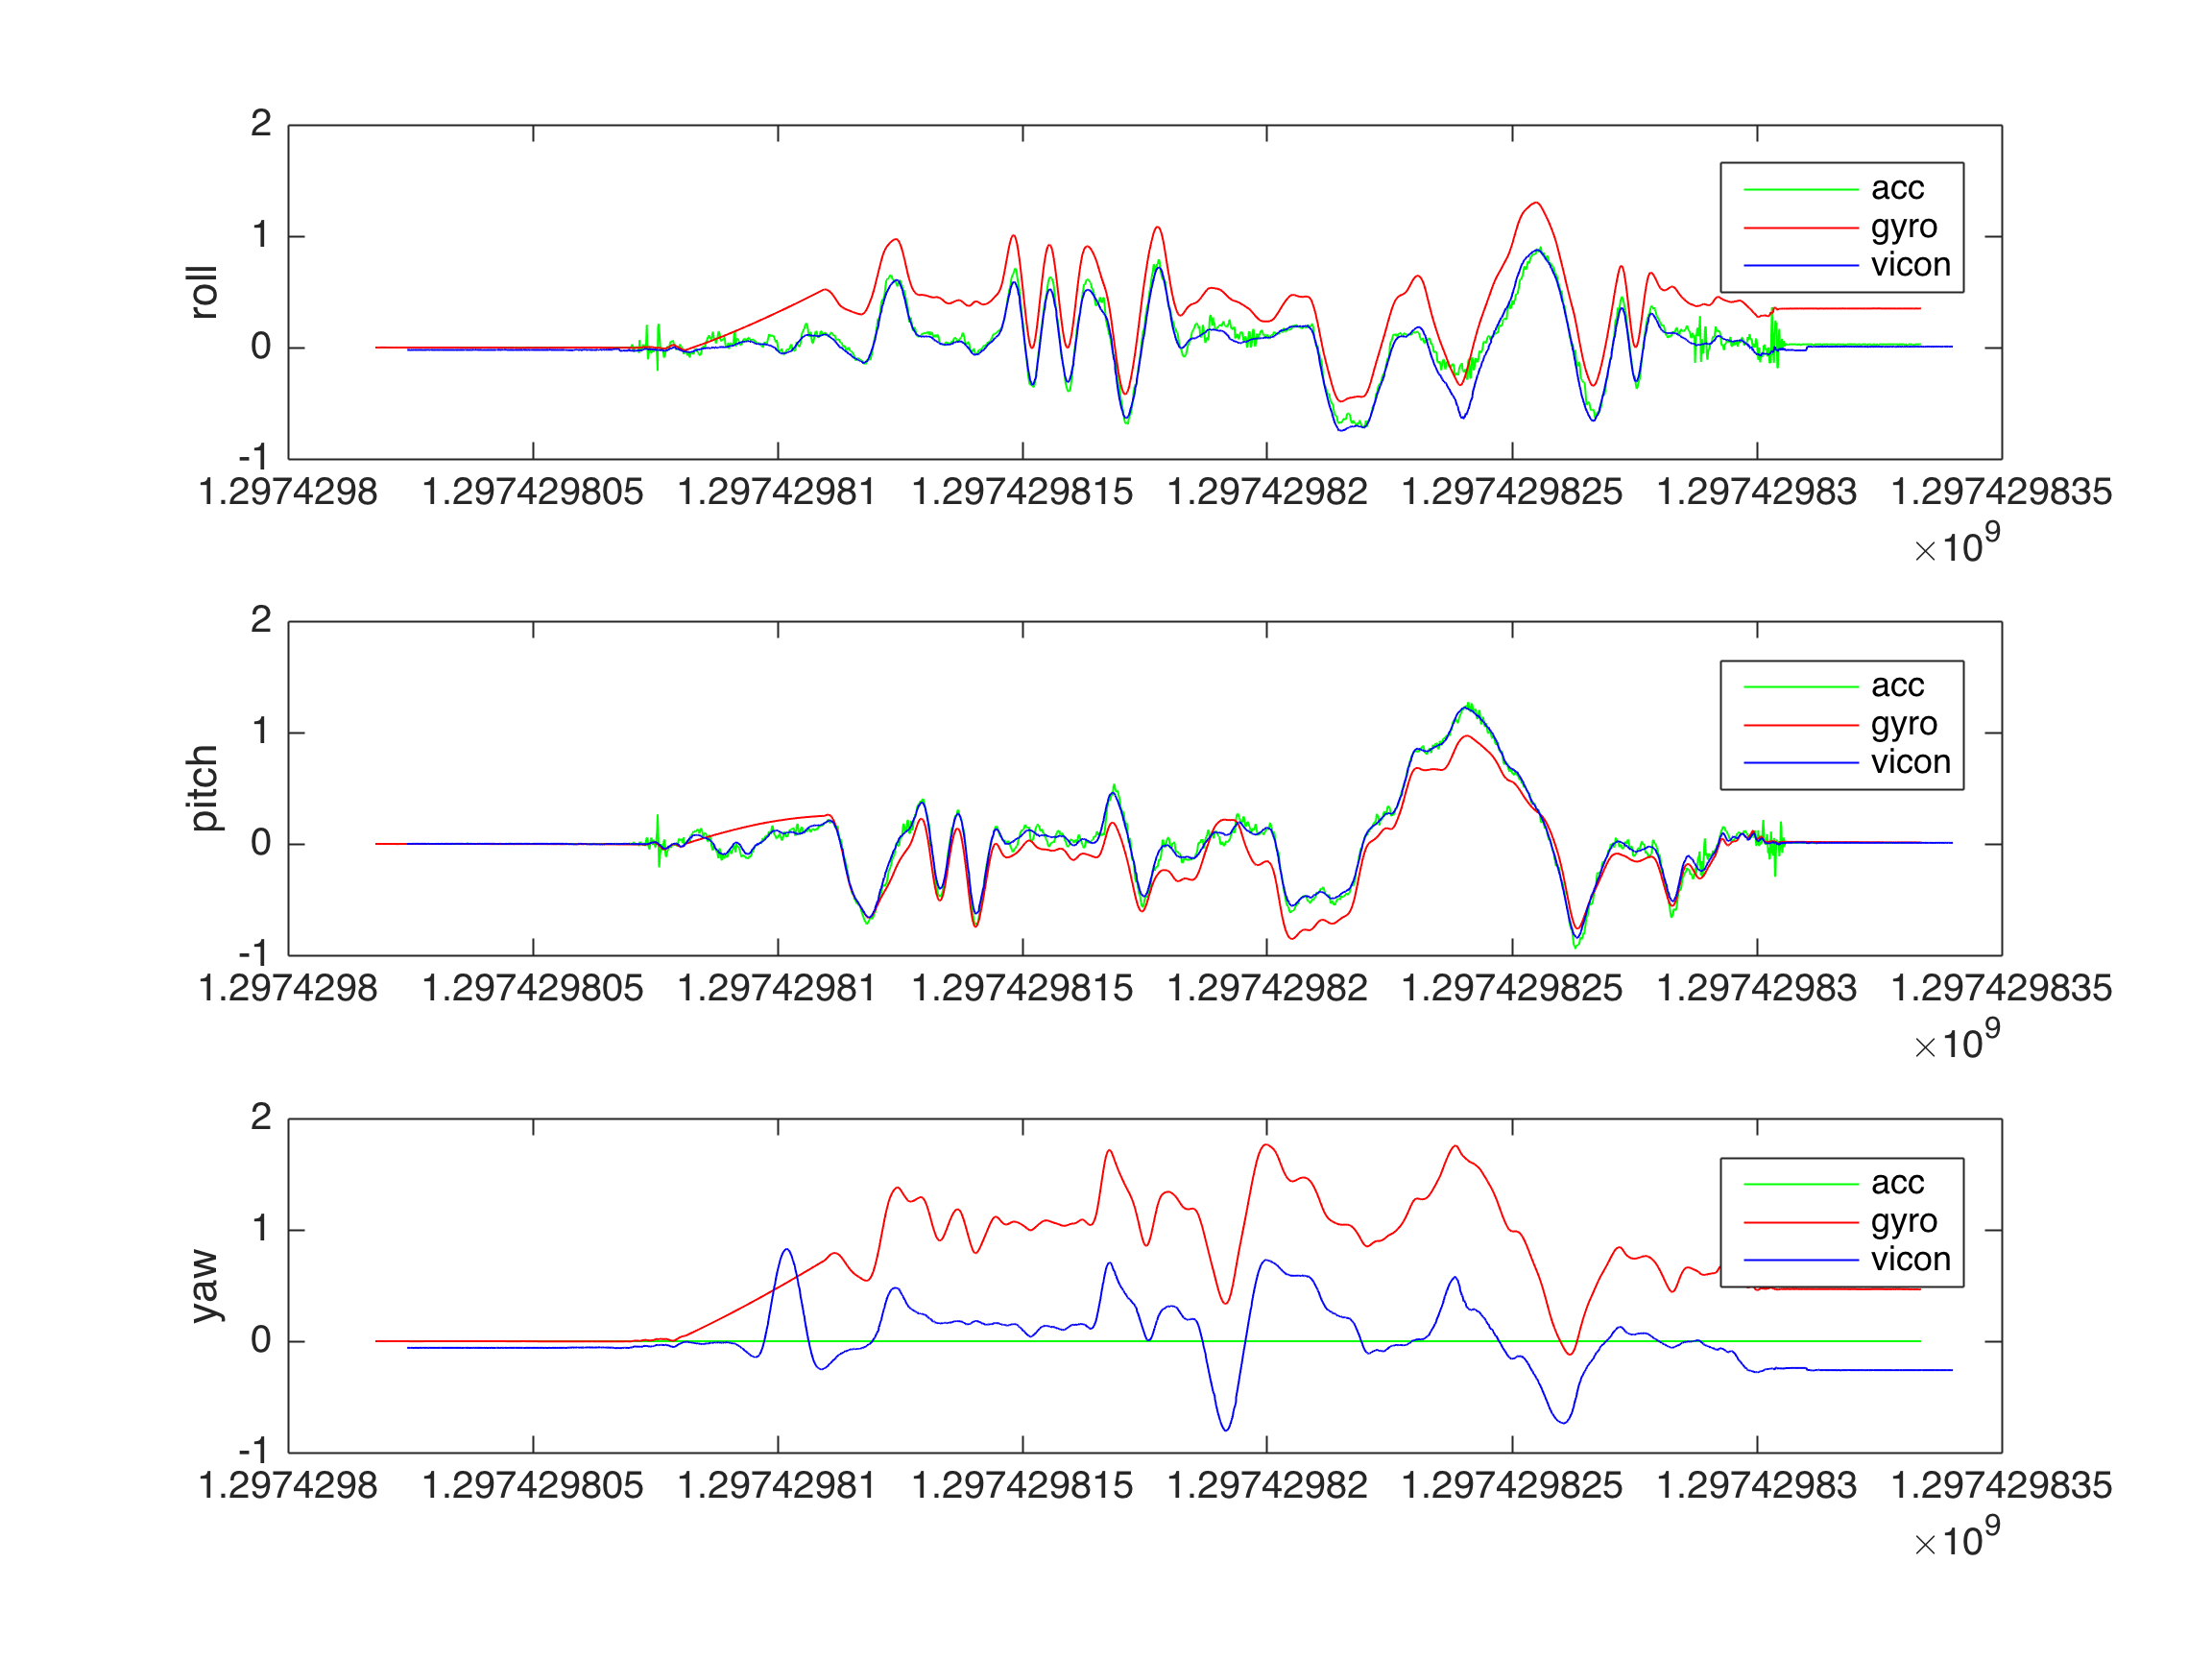
\includegraphics[scale=0.5]{images/naive_approach_4.png} 
\caption{Naive Approach from Acc and Gyro's Estimation on dataset 4}
\label{fig:naive_4}
\end{figure}

\begin{figure}
\centering
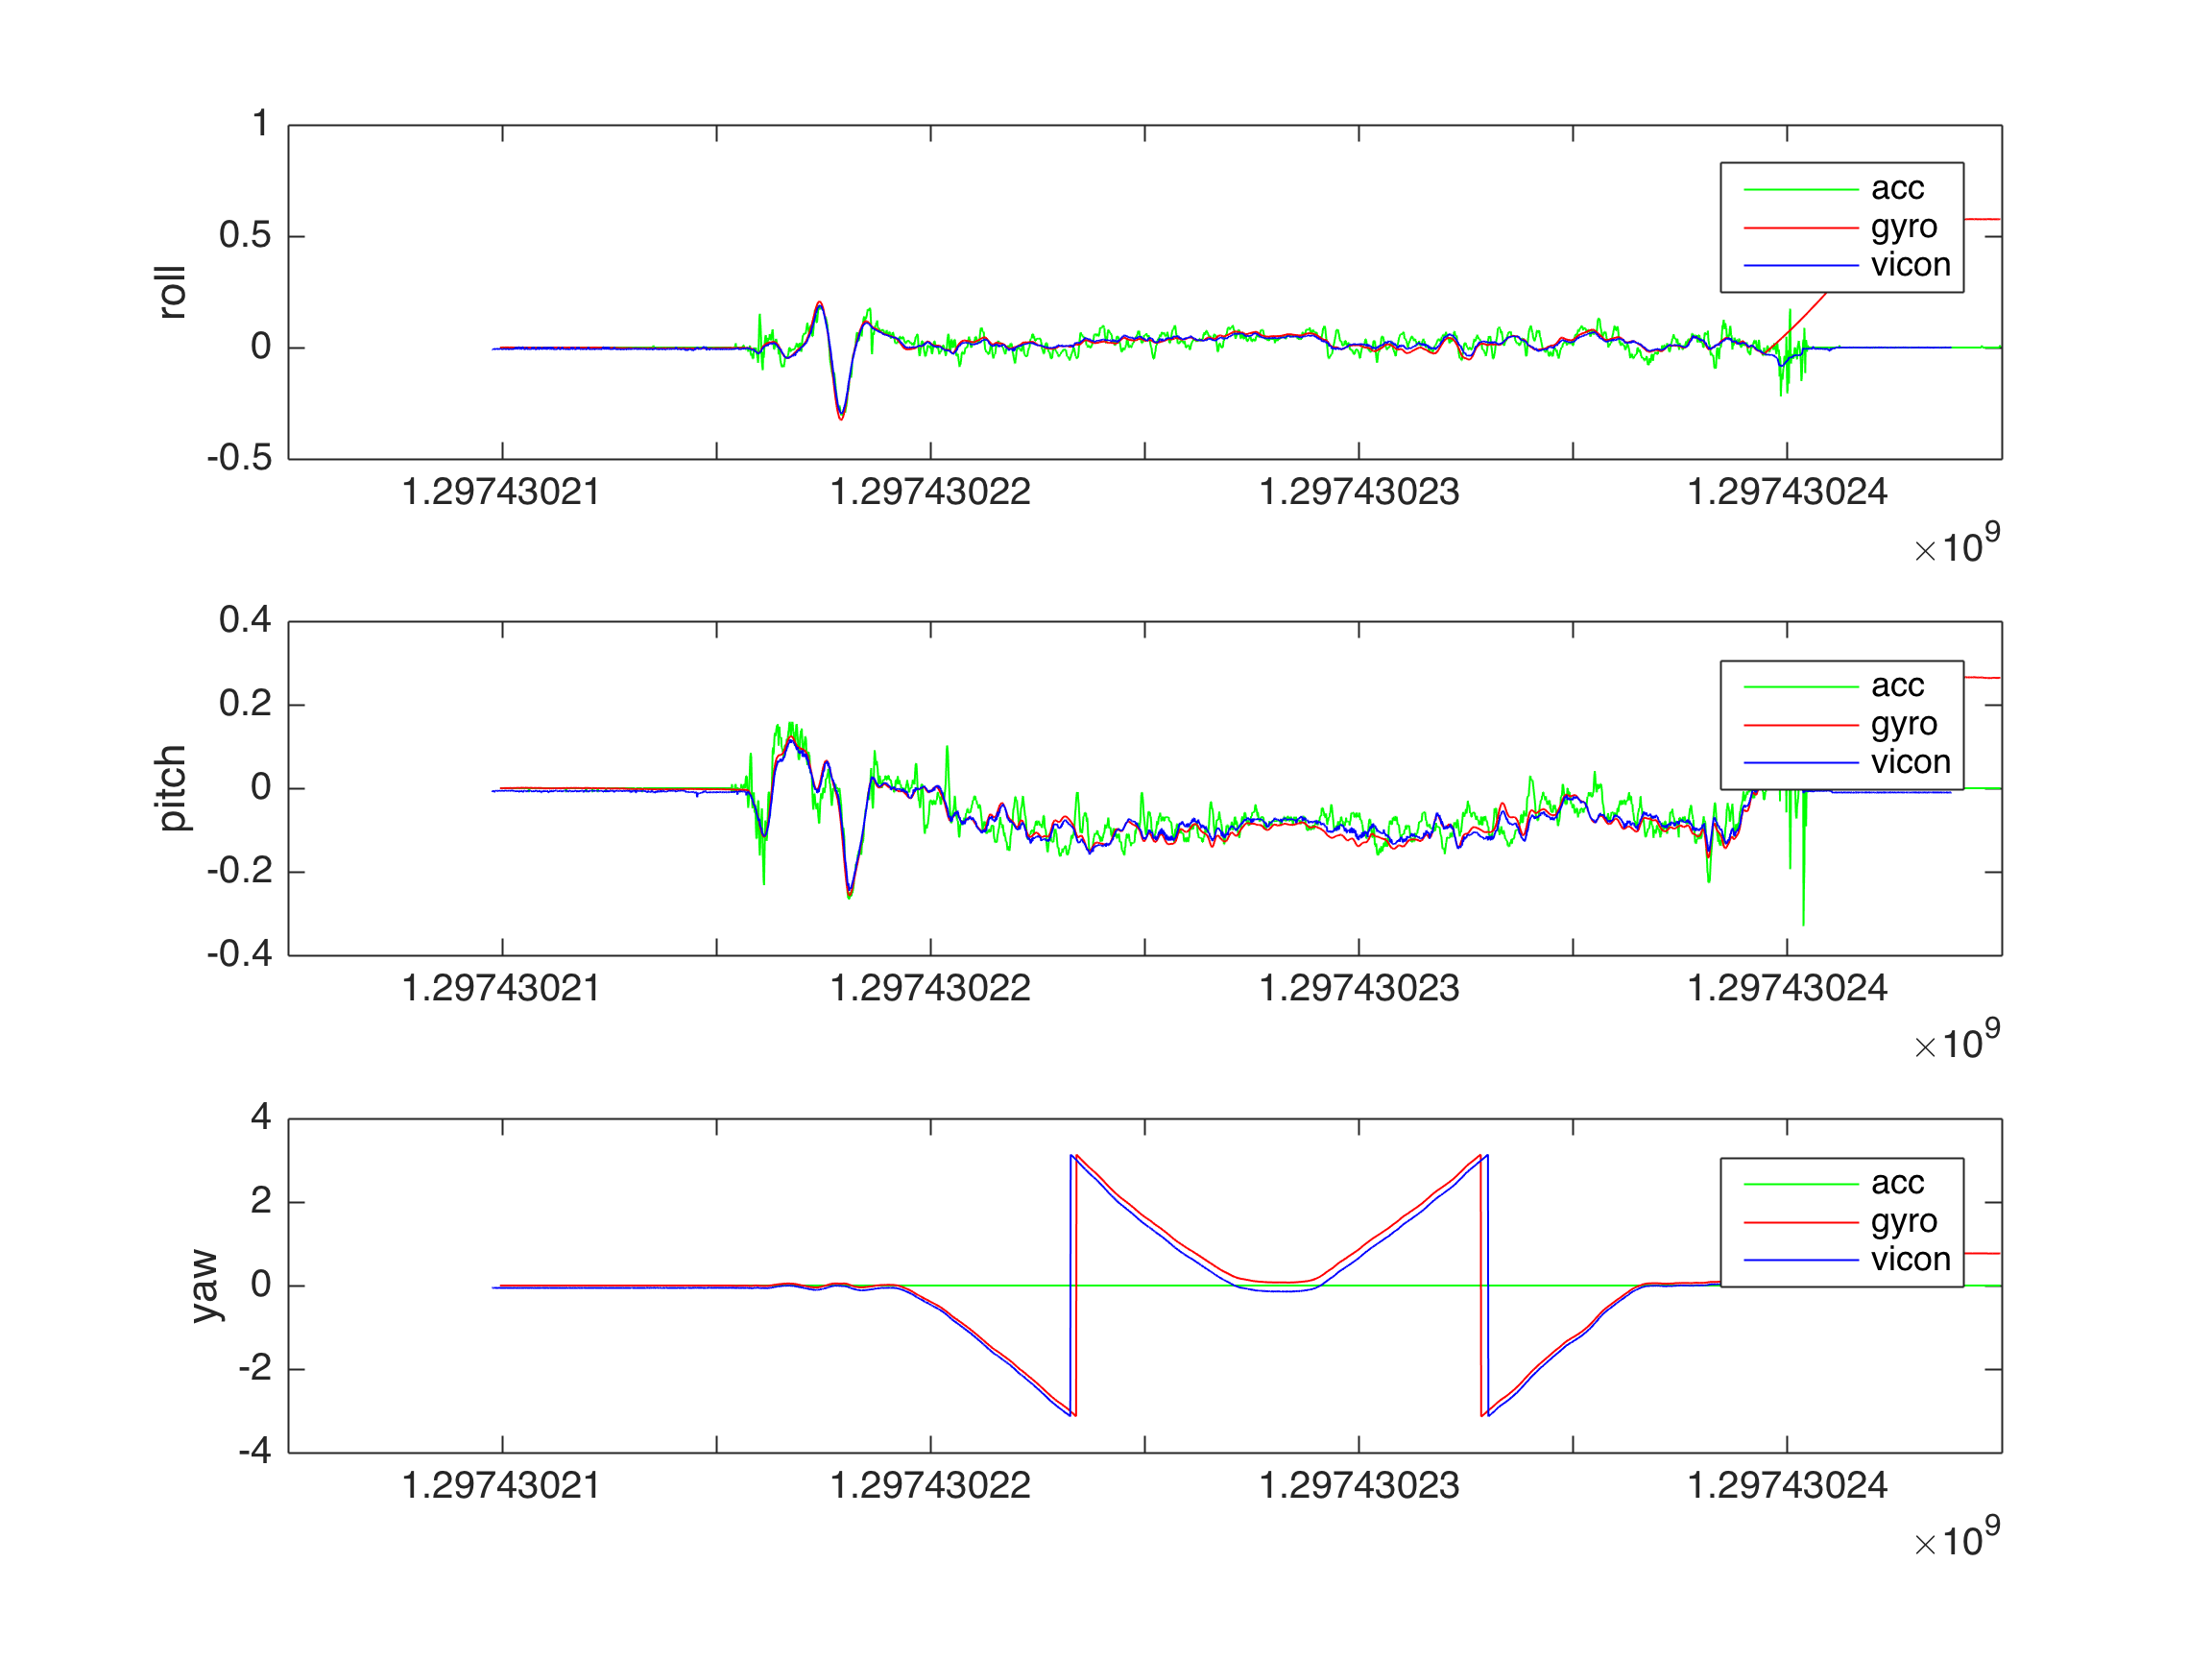
\includegraphics[scale=0.5]{images/naive_approach_8.png} 
\caption{Naive Approach from Acc and Gyro's Estimation on dataset 8}
\label{fig:naive_8}
\end{figure}

\subsection {Unscented Kalman Filter}
Kalman Filter (KF) is widely applied in a variety of technologies. While, the basic KF could only serve linear system. Extend Kalman Filter (KF) resolved this issue by linearize the nonlinear transformation by Taylor series expanion. Unscented Kalman Filter (UKF) \cite{UKF97} skipped the \emph{jacobian} operations in EKF by propagating the distribution through nonlinear tranformation on a set of so-called \emph{Sigma Points}. In this project, I implemented a UKF to gain more robust performance. \\
I implemented both a standard 7-state UKF and a 4-state UKF. The detailed algorithm for the 7-state UKF algorithm for orientation tracking refers to \cite{Kraft03}. 
\subsubsection{4-State UKF}
The 4-state vector contains a single quaternion:
\begin{align}
s_0 = [1, 0, 0, 0]^T
\end{align}
\emph{Process Model} \\
The process model is simply:
\begin{align}
s_{k+1} = (q_k q\Delta )
\end{align}
where, $q\Delta$ is generated from angular velocity and time duration as stated in 2.2.\\
\emph{Measurement Model} \\
\begin{align}
\vec z_{acc} = q_k g q_k^{-1} + \vec v_{acc}
\end{align}
where, $g = [0,0,0,1]$ representing the gravity.\\
All the other parts of the algorithm are the same as 7-state UKF. In my implementation, I found that the 4-state UKF actually works better in most cases. Thus, the results being shown in this reports are all generated from 4-state UKF.

\subsection {Fuse UKF with Gryo's}
For my implementation, I find that the results my algorithm produces is mainly affected by the Accelerometer's prediction, which works poorly on \emph{yaw} angle. Since the yaw prediction of Gyroscope works really well. I fused the $roll$ and $pitch$ prediction of UKF with Gyro's $yaw$ angles. The results could be seen in Figure \ref{fig:fuse_8}.


\begin{figure}
\centering
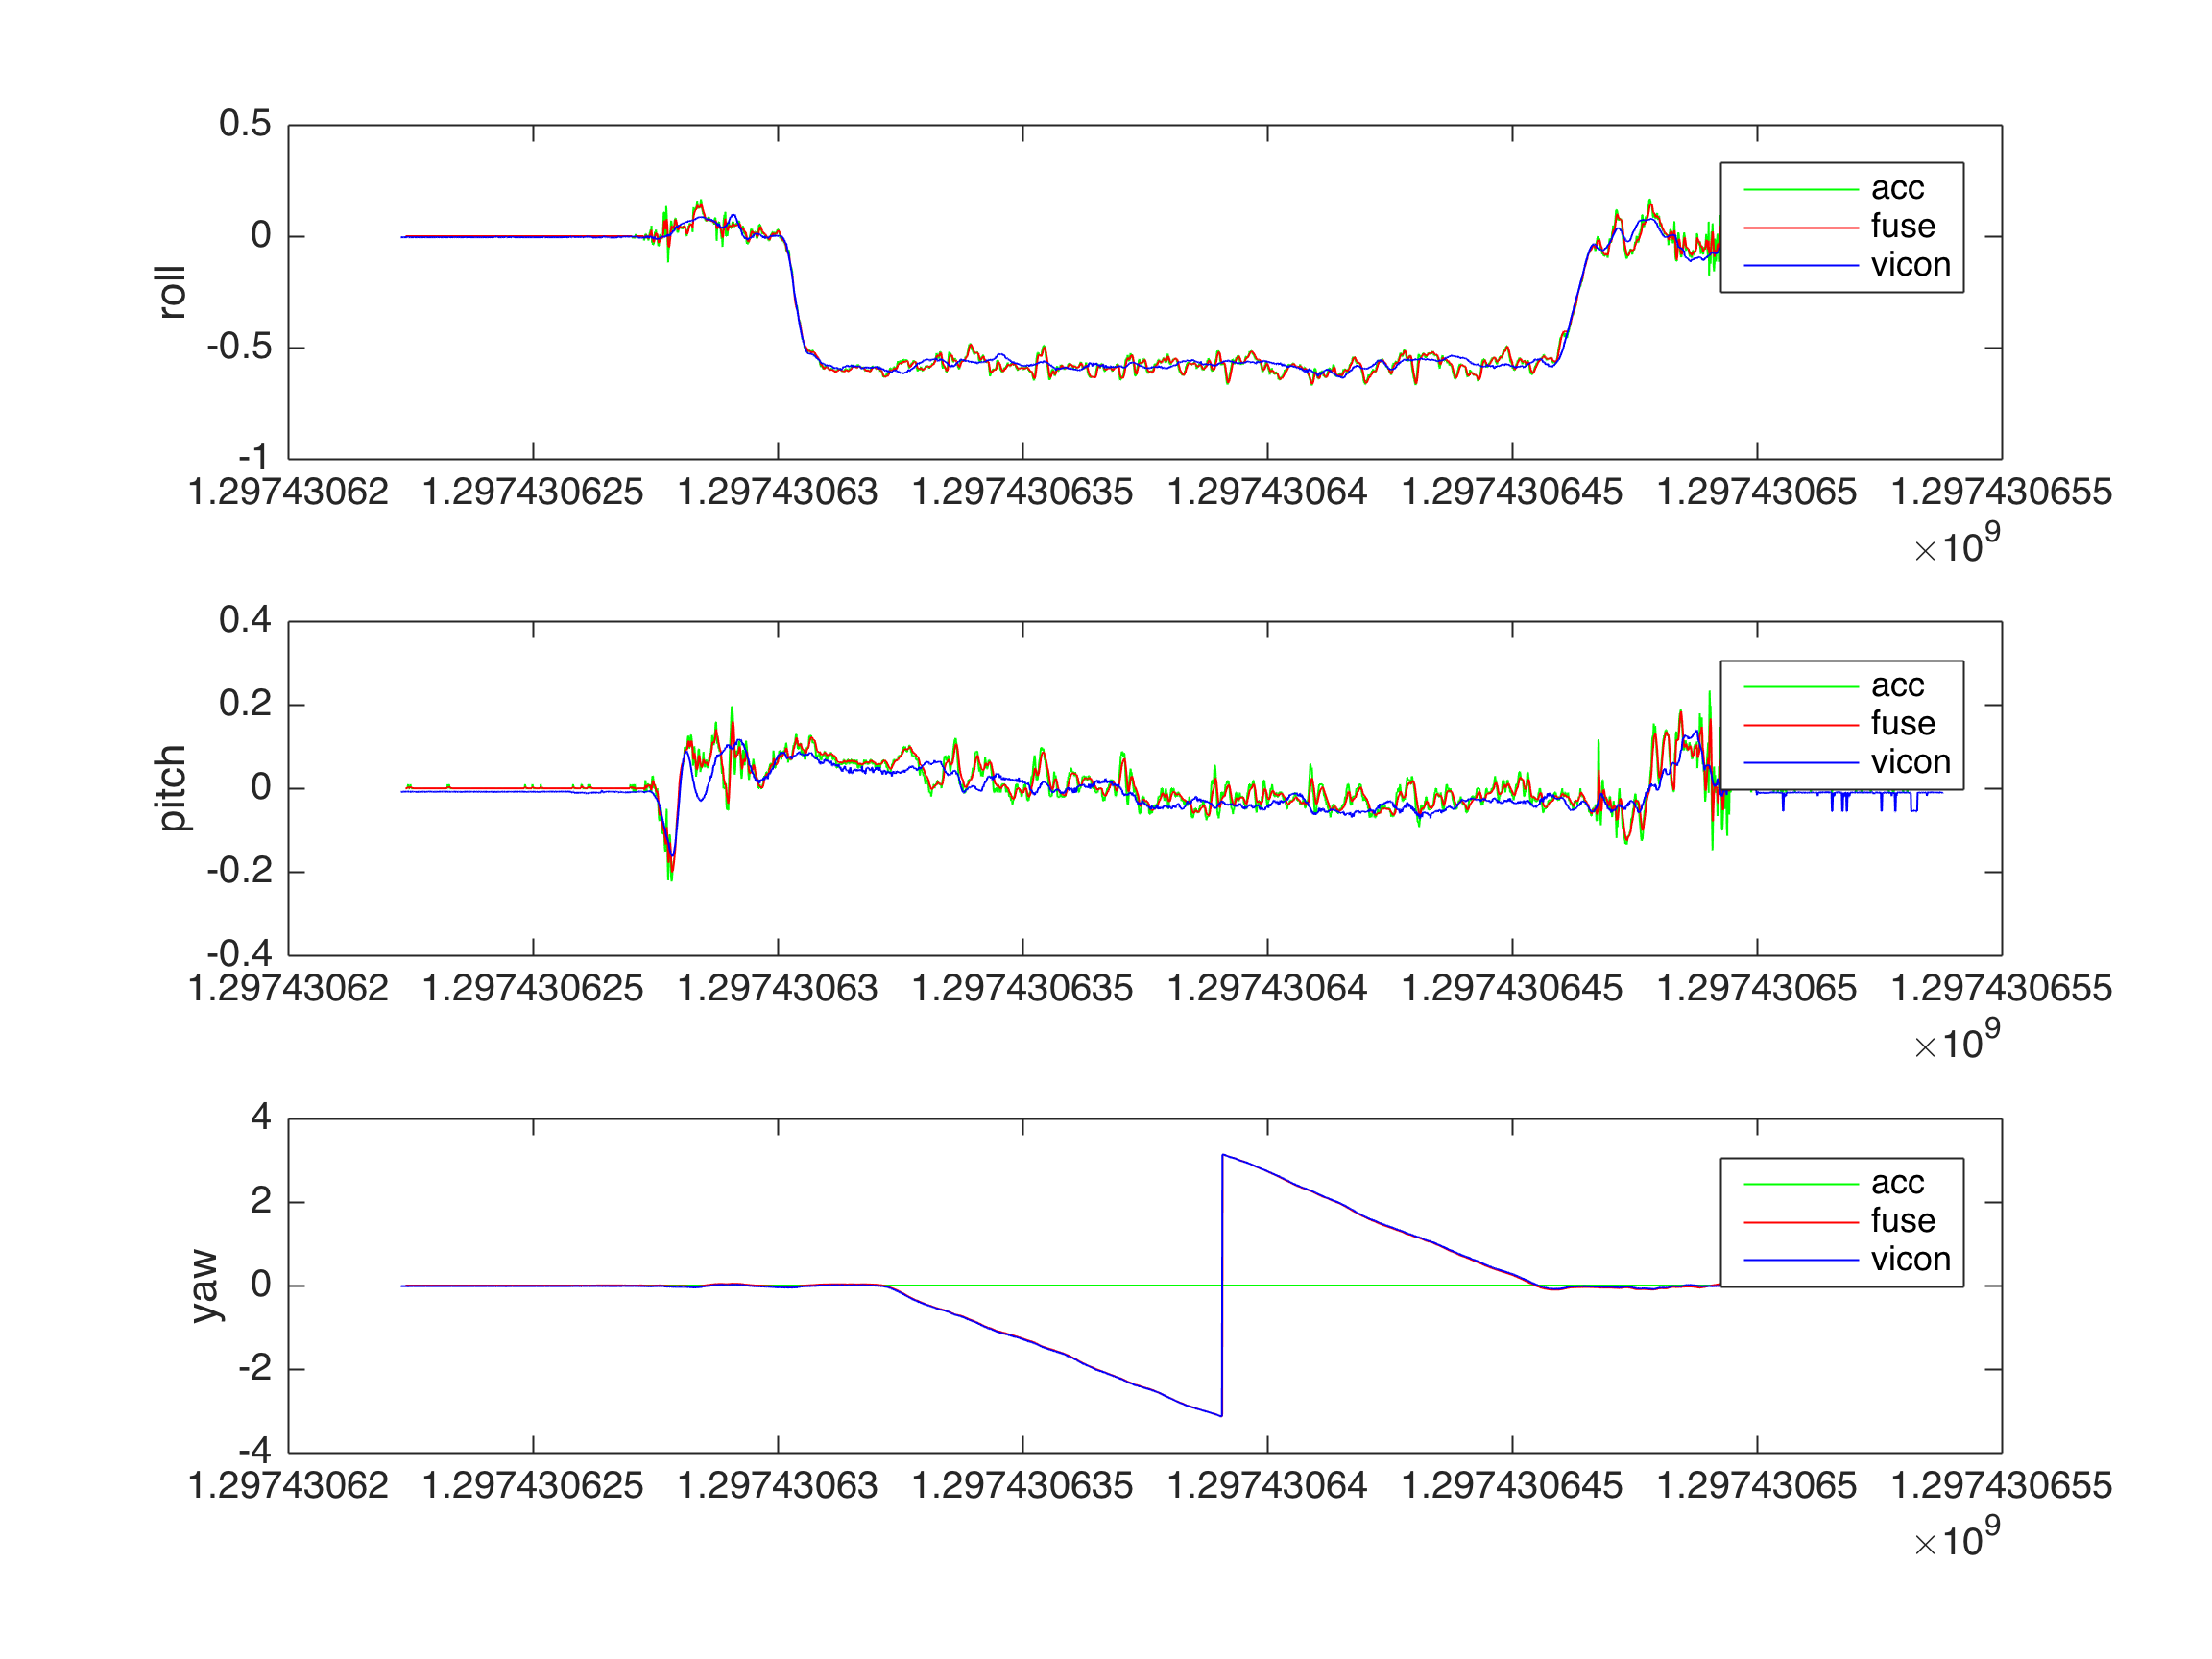
\includegraphics[scale=0.5]{images/Fuse_100.png} 
\caption{Fusion on dataset 8}
\label{fig:fuse_8}
\end{figure}



\section {Image Stitching}
\begin{figure}
\centering
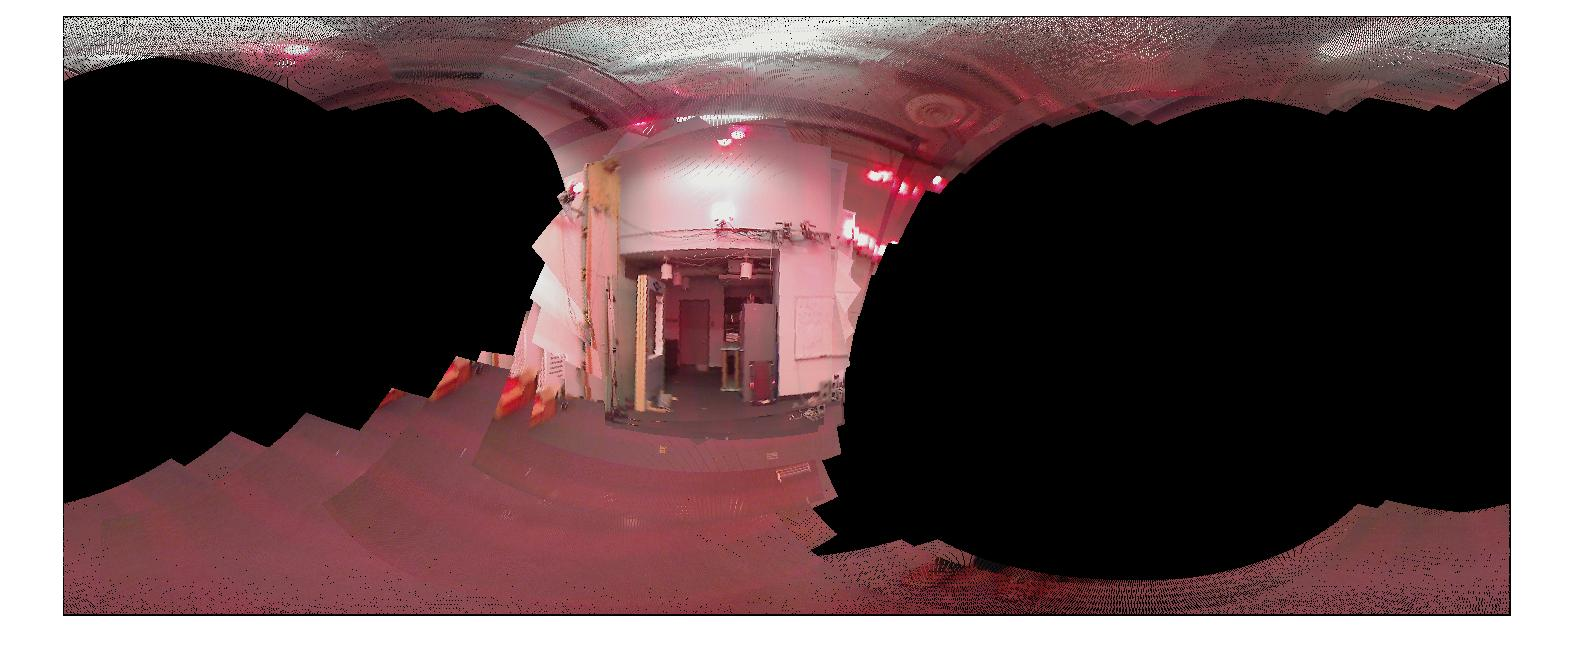
\includegraphics[scale=0.2]{images/pano2.jpg} 
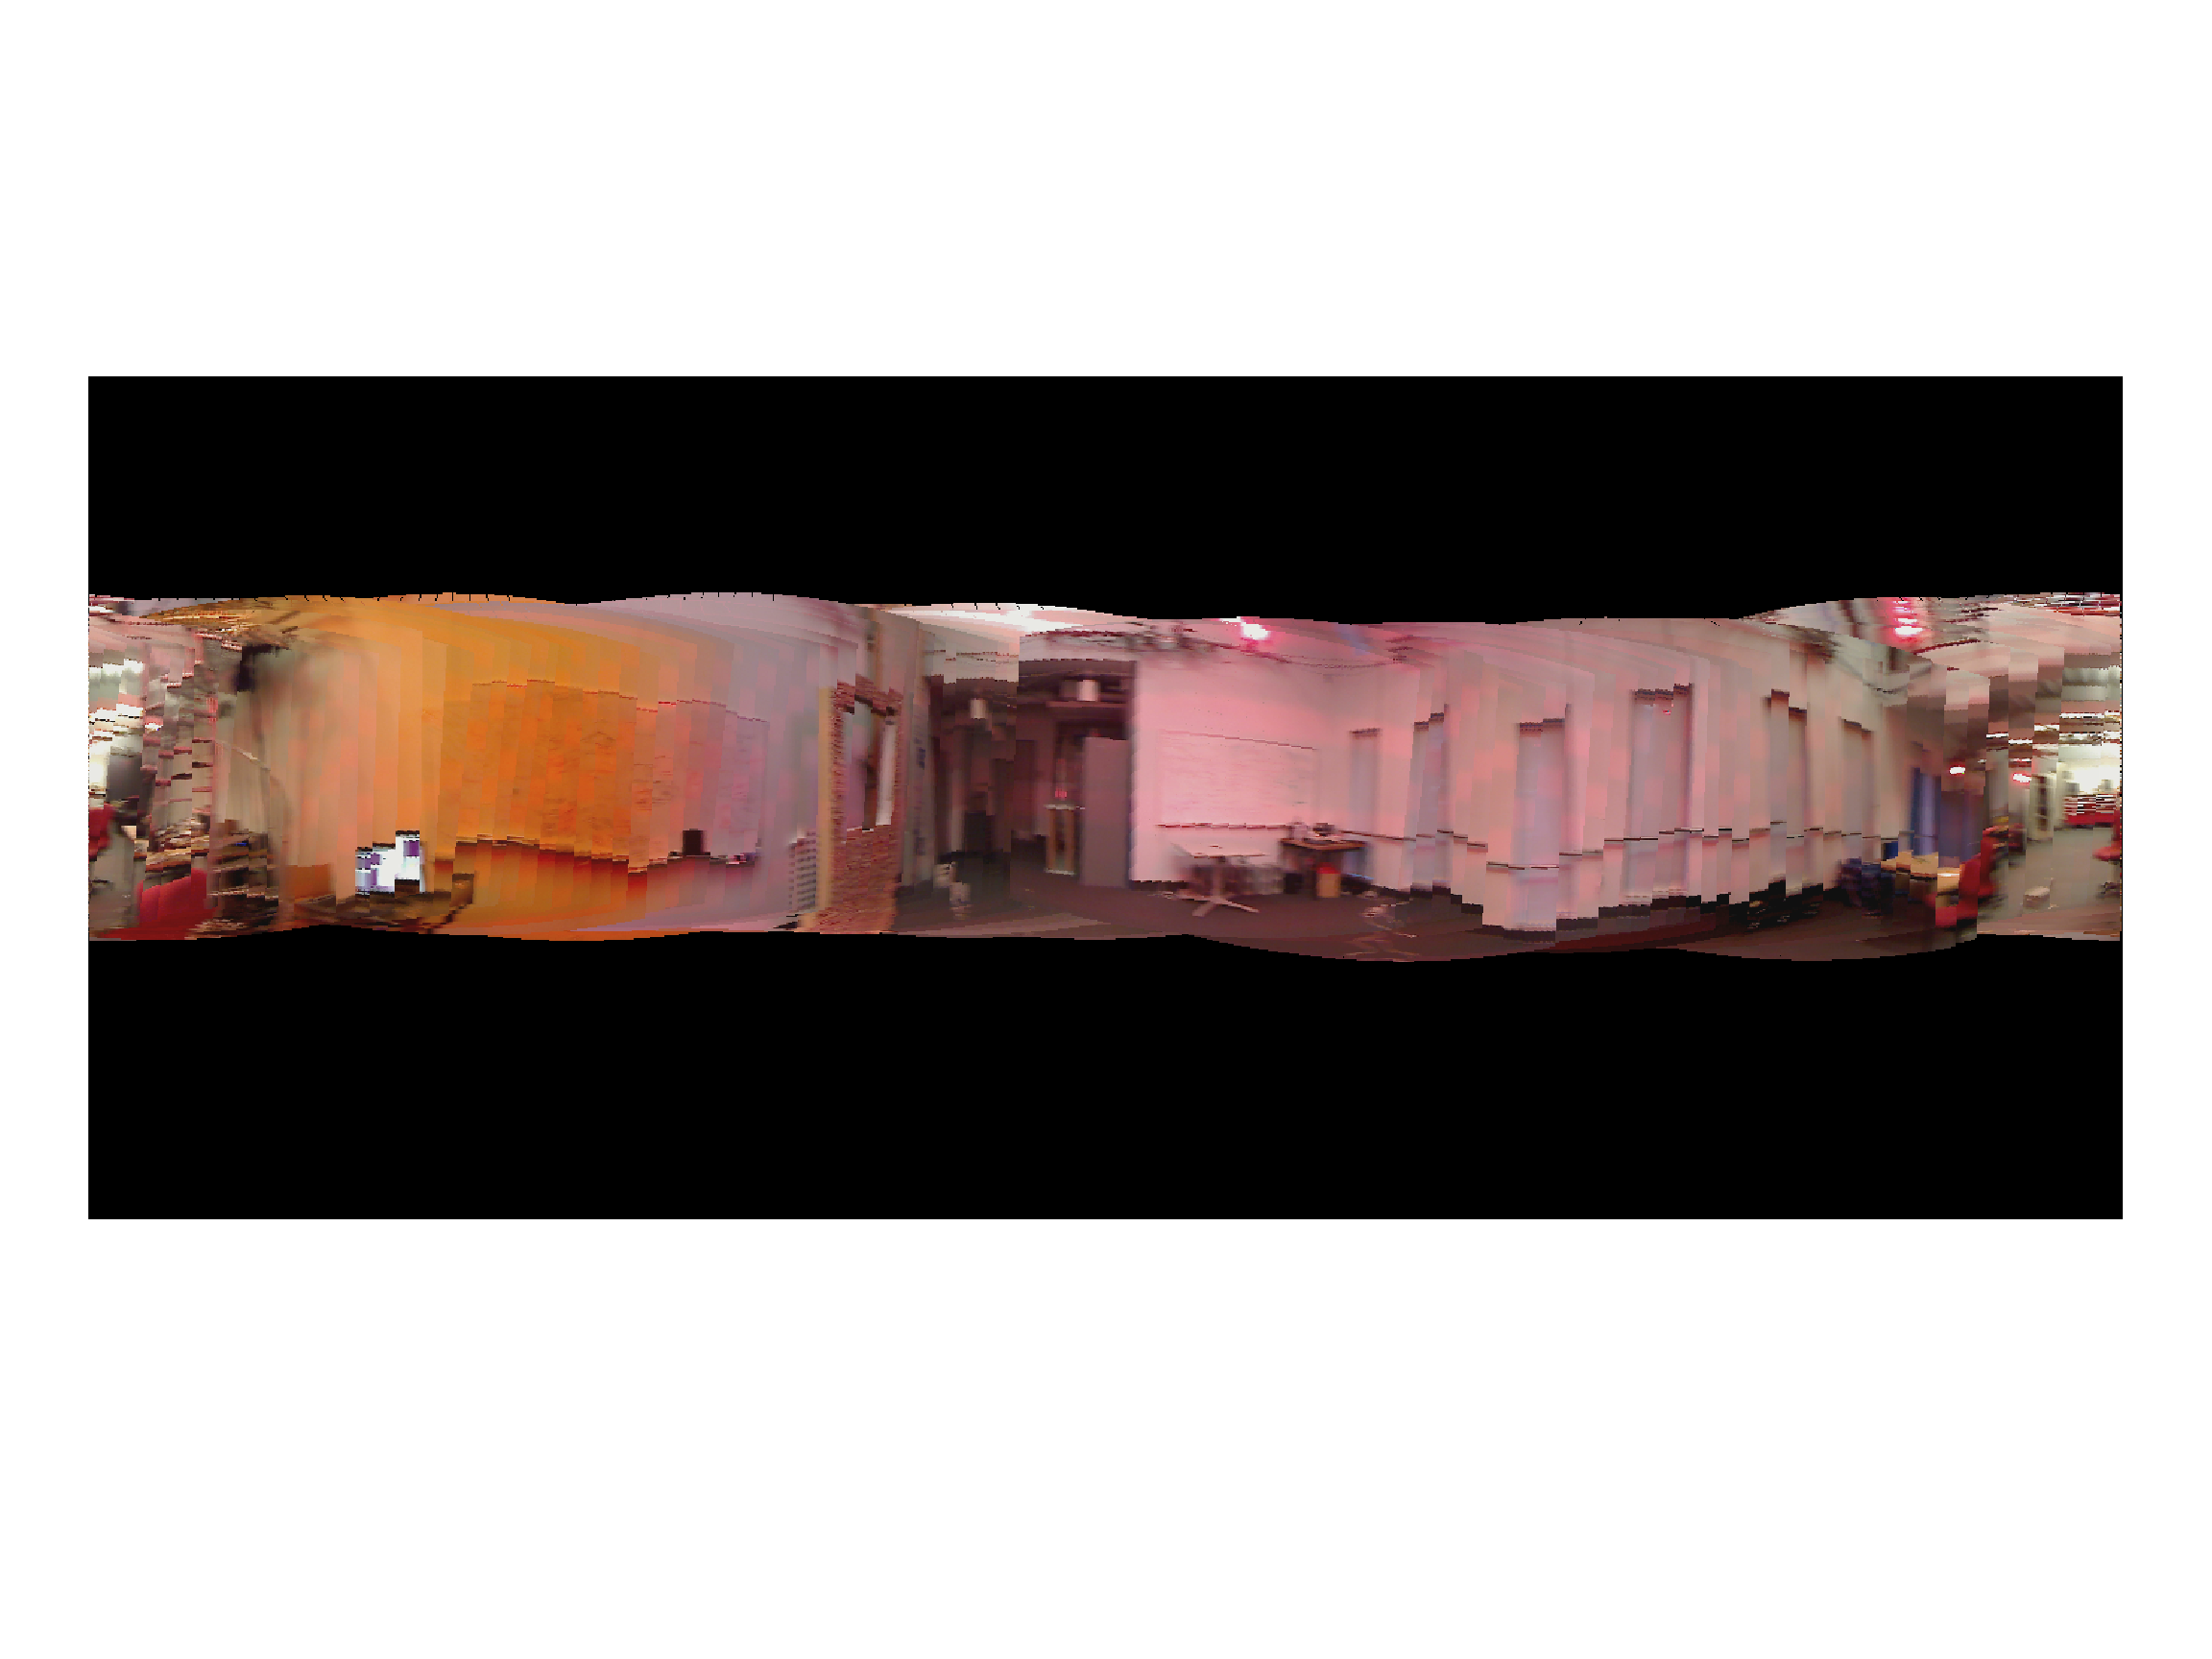
\includegraphics[scale=0.5]{images/pano8.png} 
\caption{Panoramic Image of Dataset 2 and 8}
\label{fig:pano}
\end{figure}

For image stitching, I found an algorithm that project 3-D points into cylindral coordinate and then unwrap the cylinder into a panoramic image. Therefore, first assign  z coordinates to the images, and then perform rotation to the image using computed rotation matrices. After that perform the mapping and unwrapping. As shown in Figure \ref{fig:pano}. Due to time limitation, I only tried this single method.

\section {Results and Discussion}
Performing my algorithm on the test set yields the results in Figure \ref{fig:naive_test} \ref{fig:ukf_test} \ref{fig:fuse_test} \ref{fig:pano_test} 
\begin{itemize}
\item \emph{The initialization of noise covariance matrices} for process and measurement models are is important. While, in this project I didnt use methods to parameterize the covariance matrices other than trial and error. However, smaller coveriances parameters means less uncertanty. We can use this to control the performance according to our belief of the robustness for process and measurement model.
\item By \emph{fusing sensors data}, we can obtain better estimation.
\end{itemize}

\section {Acknowledgement}
Thanks Dr. Lee for designing and preparing this project and thanks TAs for timely responses to our questions.
\begin{figure}
\centering
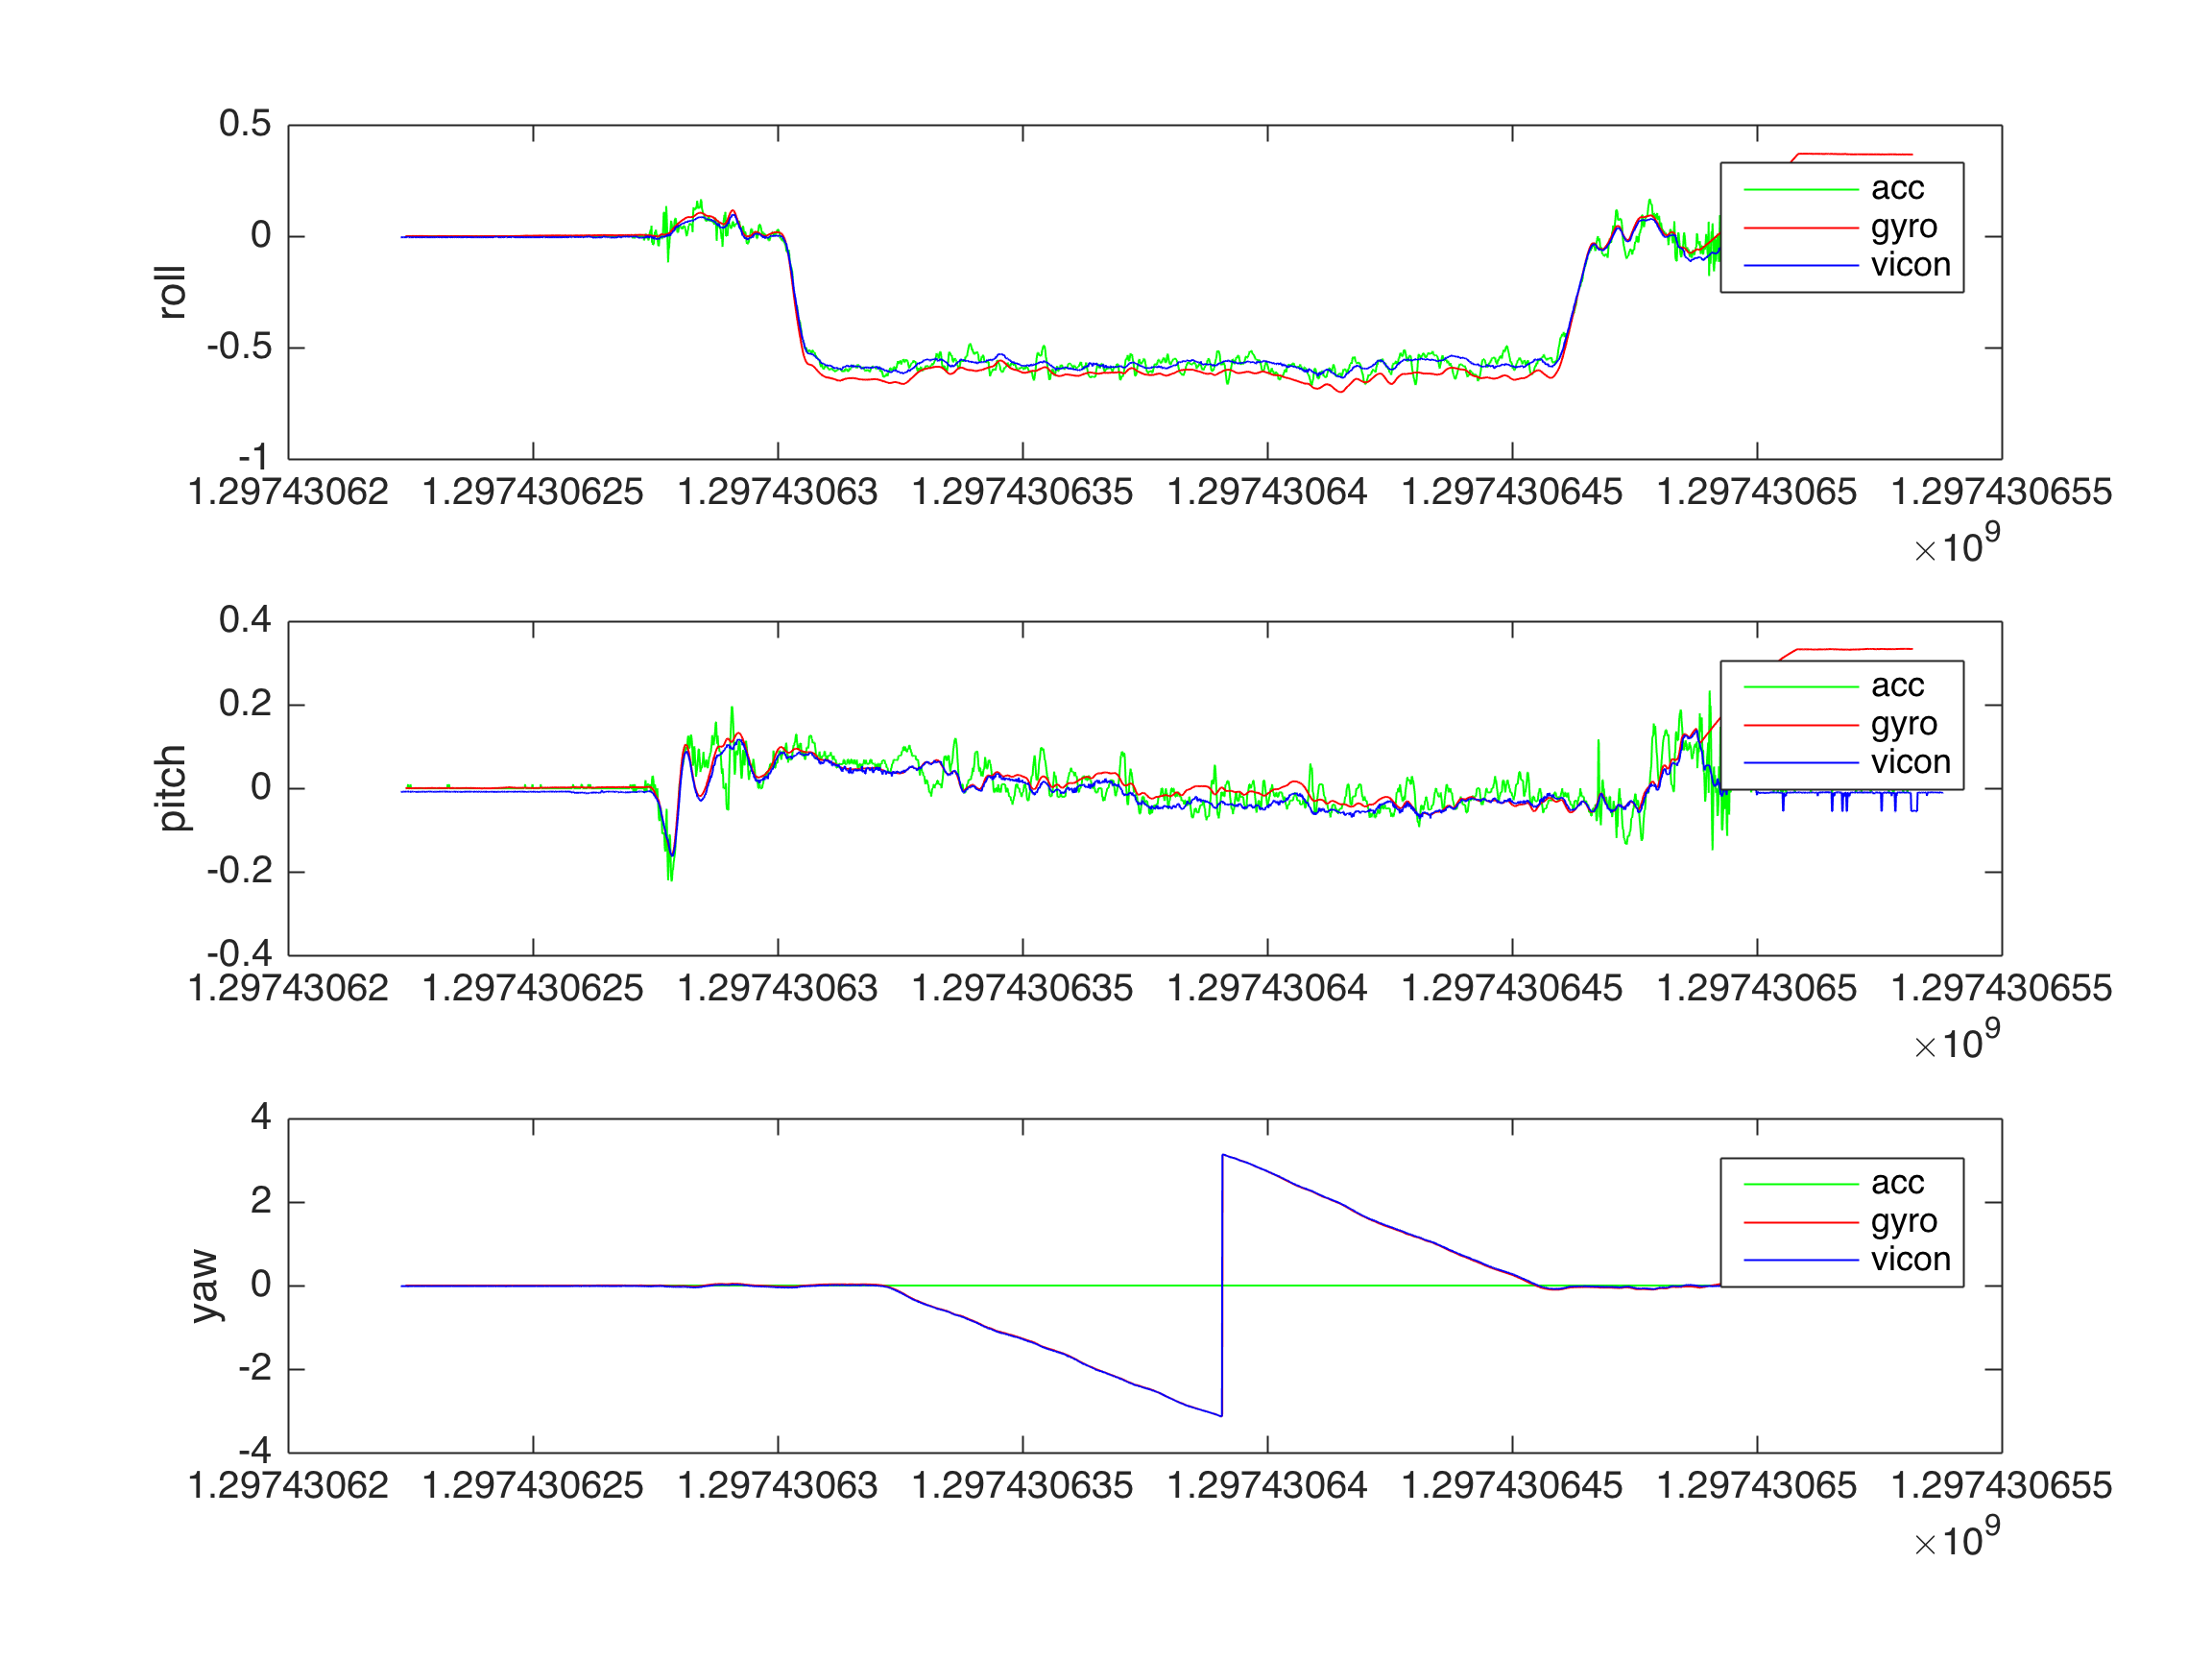
\includegraphics[scale=0.5]{images/naive_approach_100.png} 
\caption{Naive approach on test set}
\label{fig:naive_test}
\end{figure}



\begin{figure}
\centering
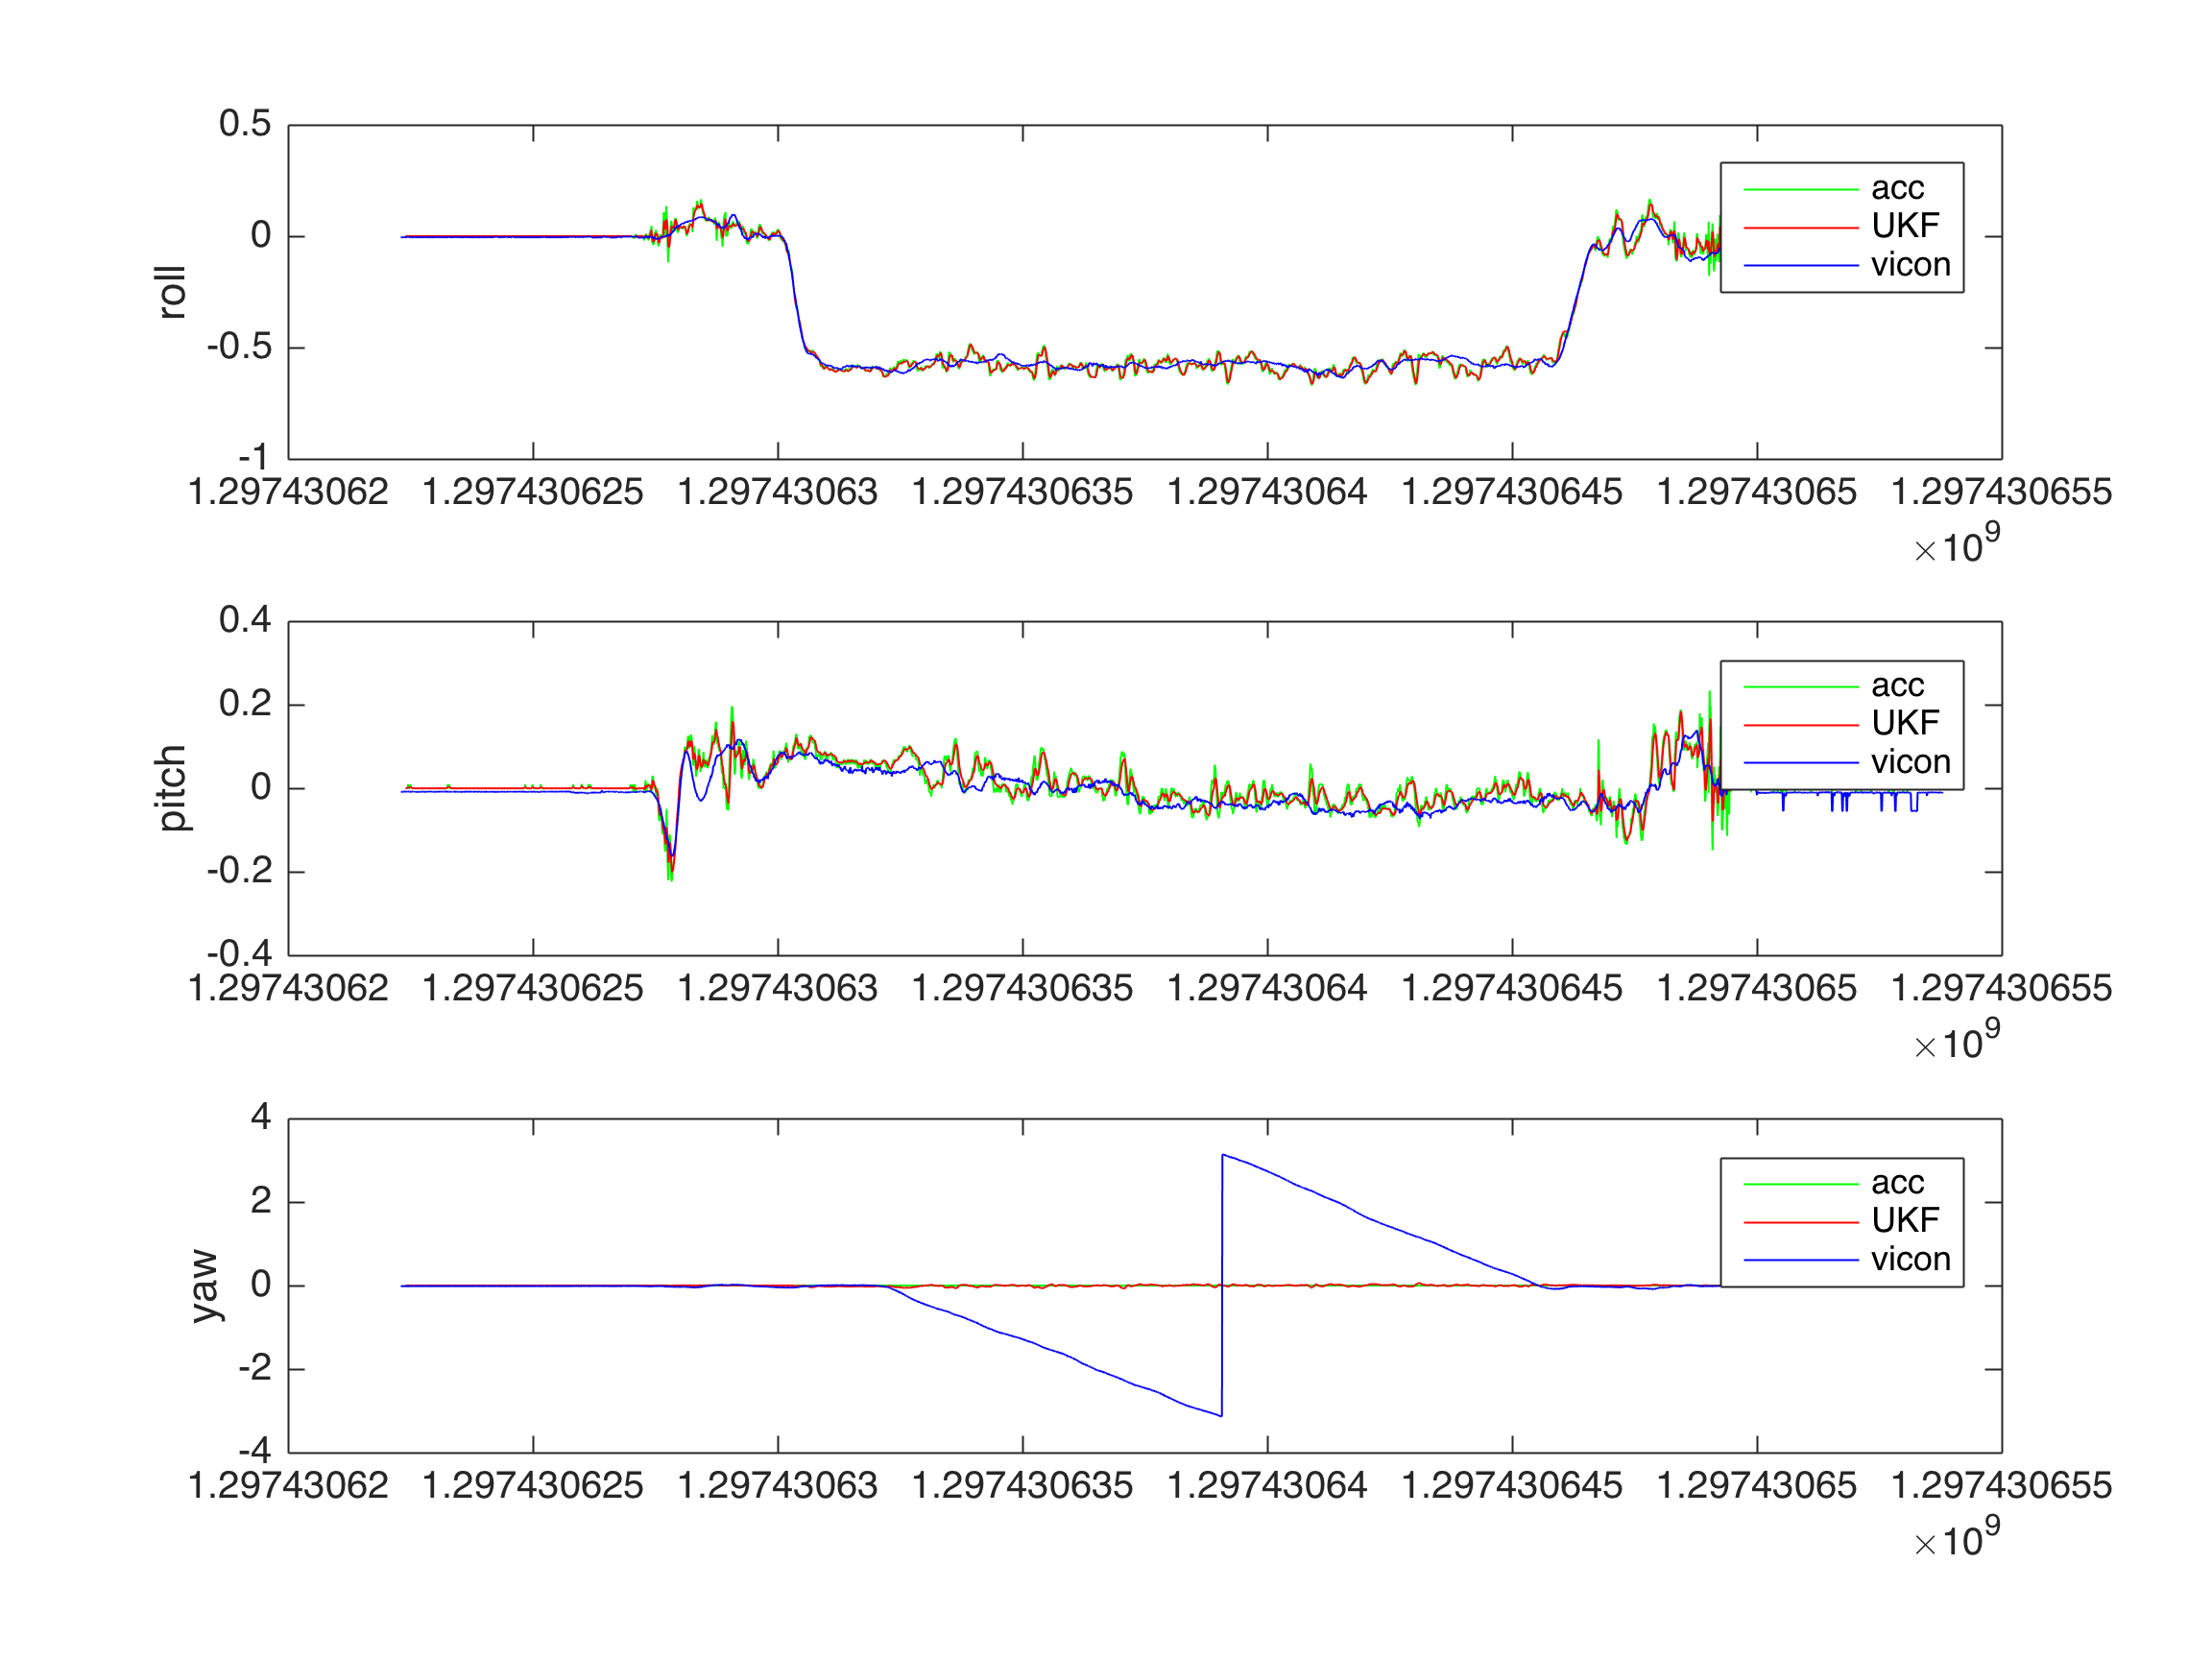
\includegraphics[scale=0.5]{images/UKF_100.png} 
\caption{UKF on test set}
\label{fig:ukf_test}
\end{figure}


\begin{figure}
\centering
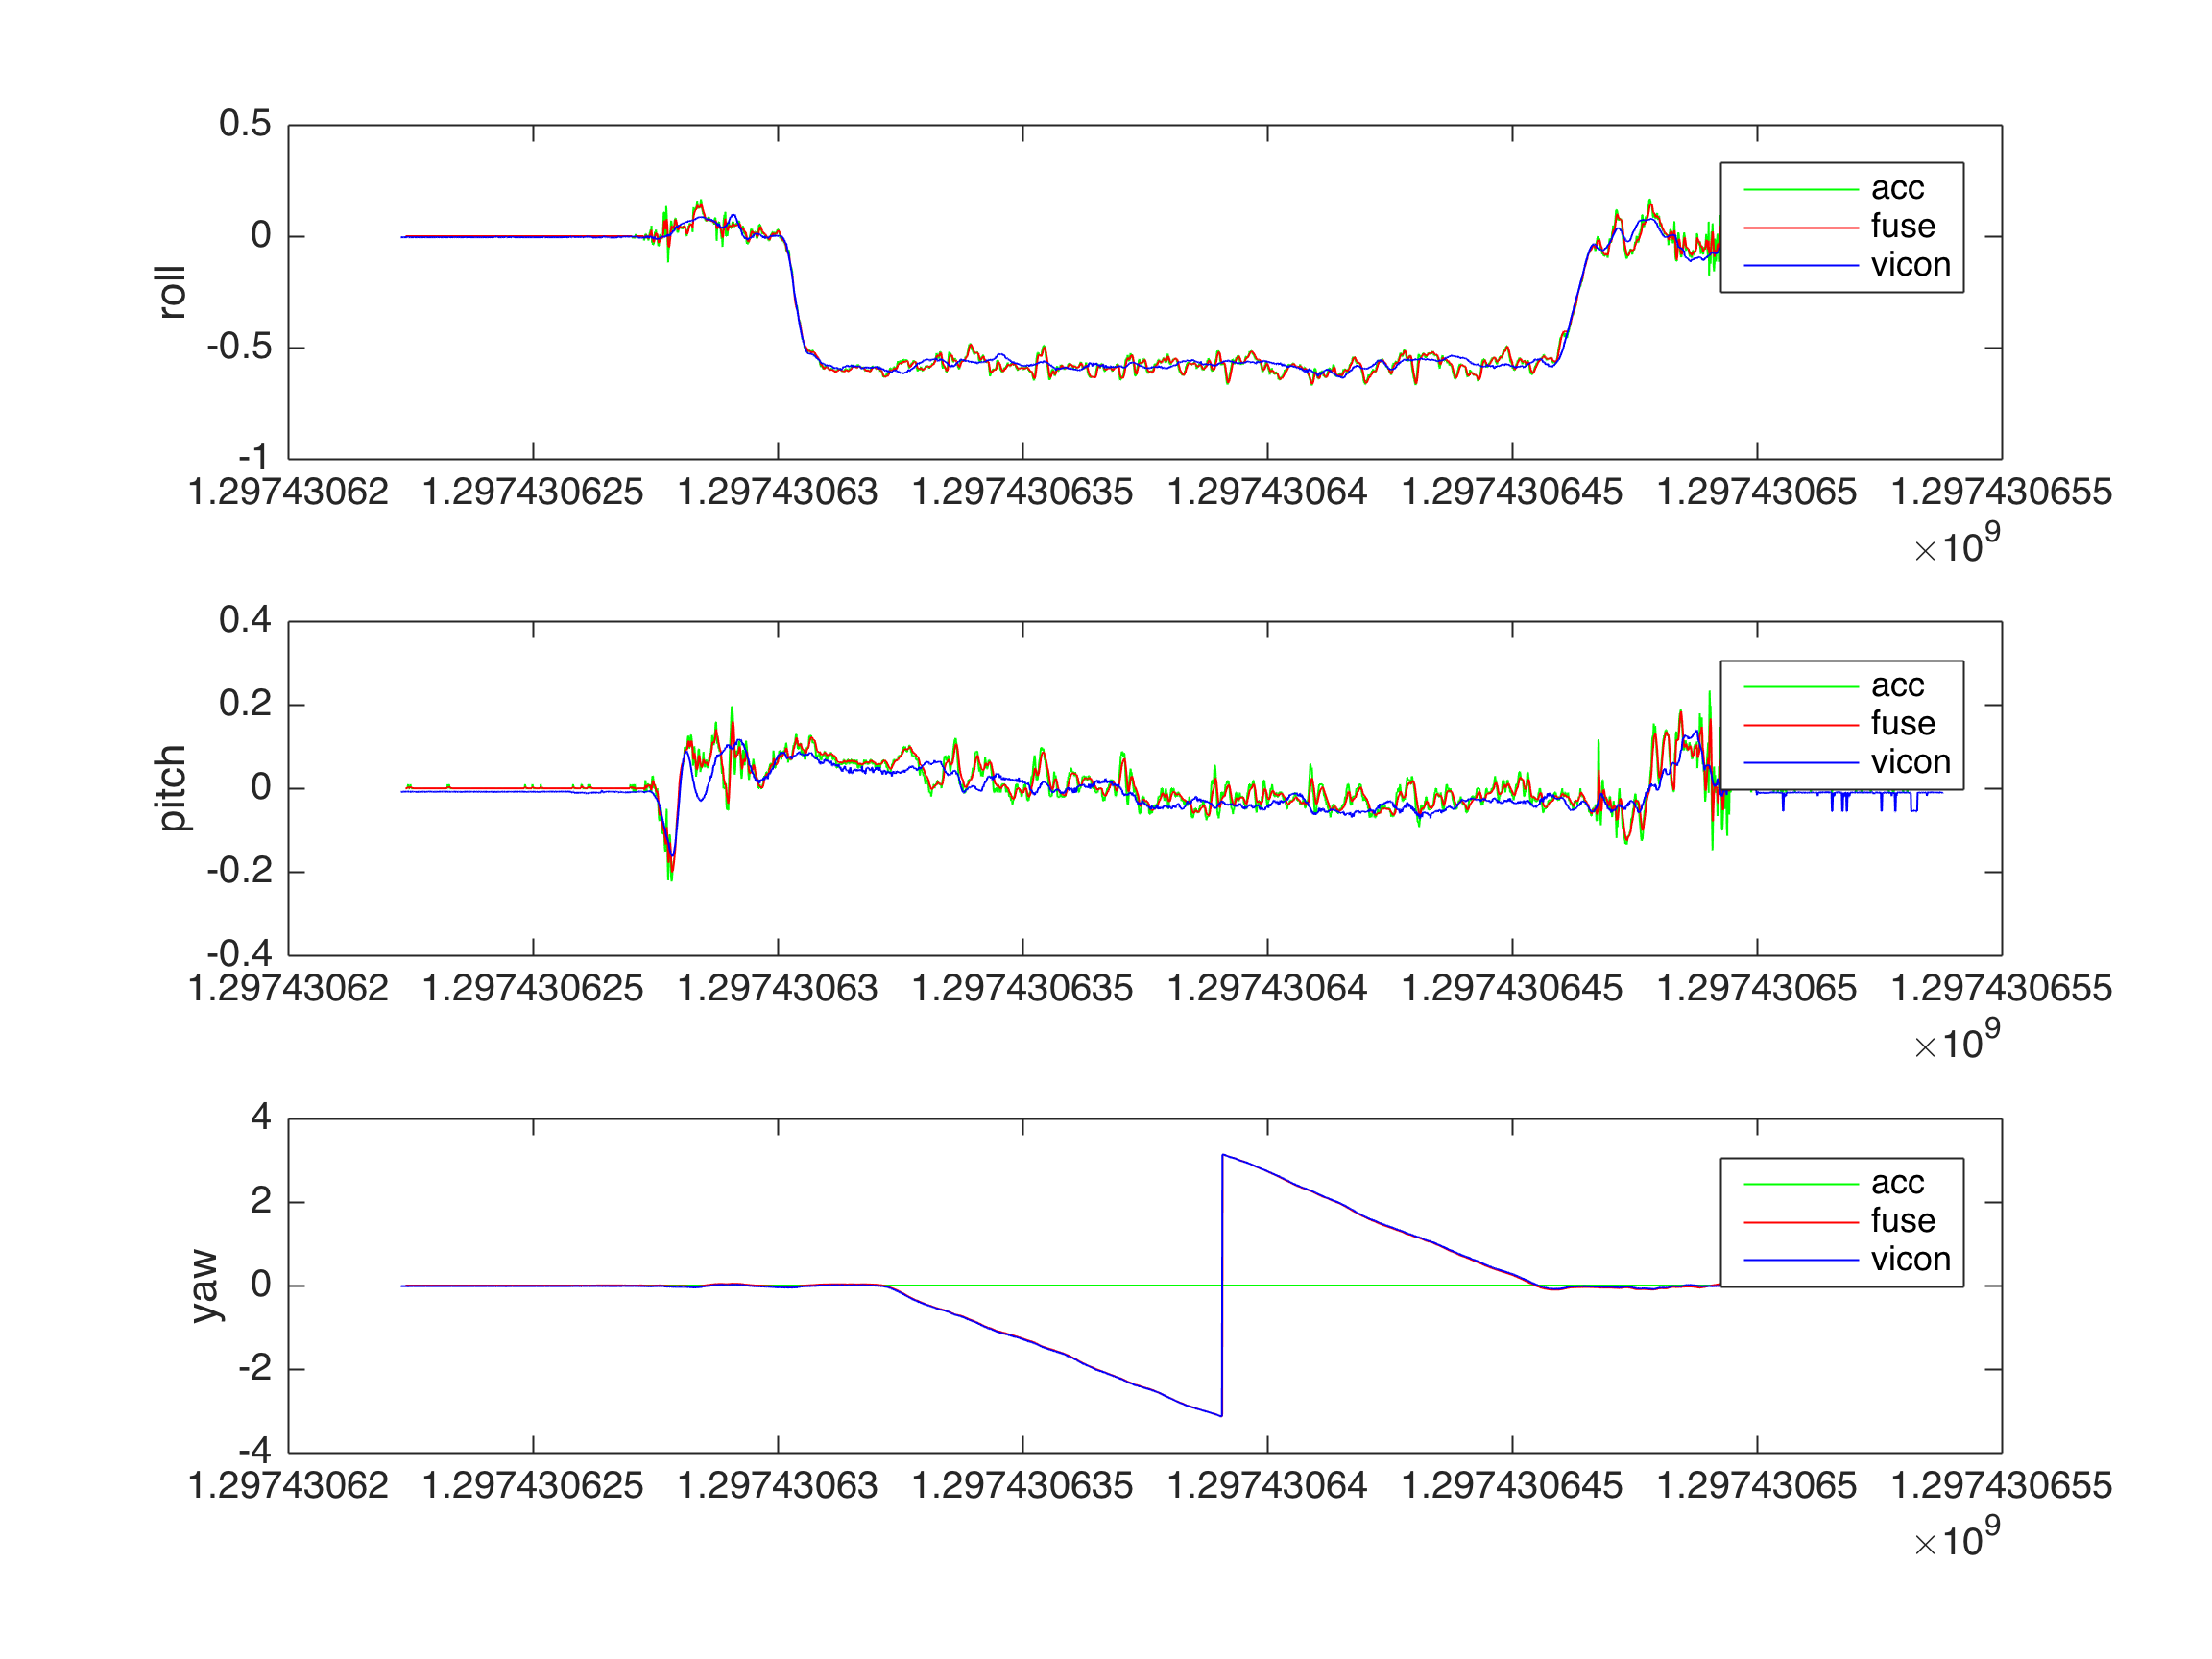
\includegraphics[scale=0.5]{images/Fuse_100.png} 
\caption{Fusion on test set}
\label{fig:fuse_test}
\end{figure}



\begin{figure}
\centering
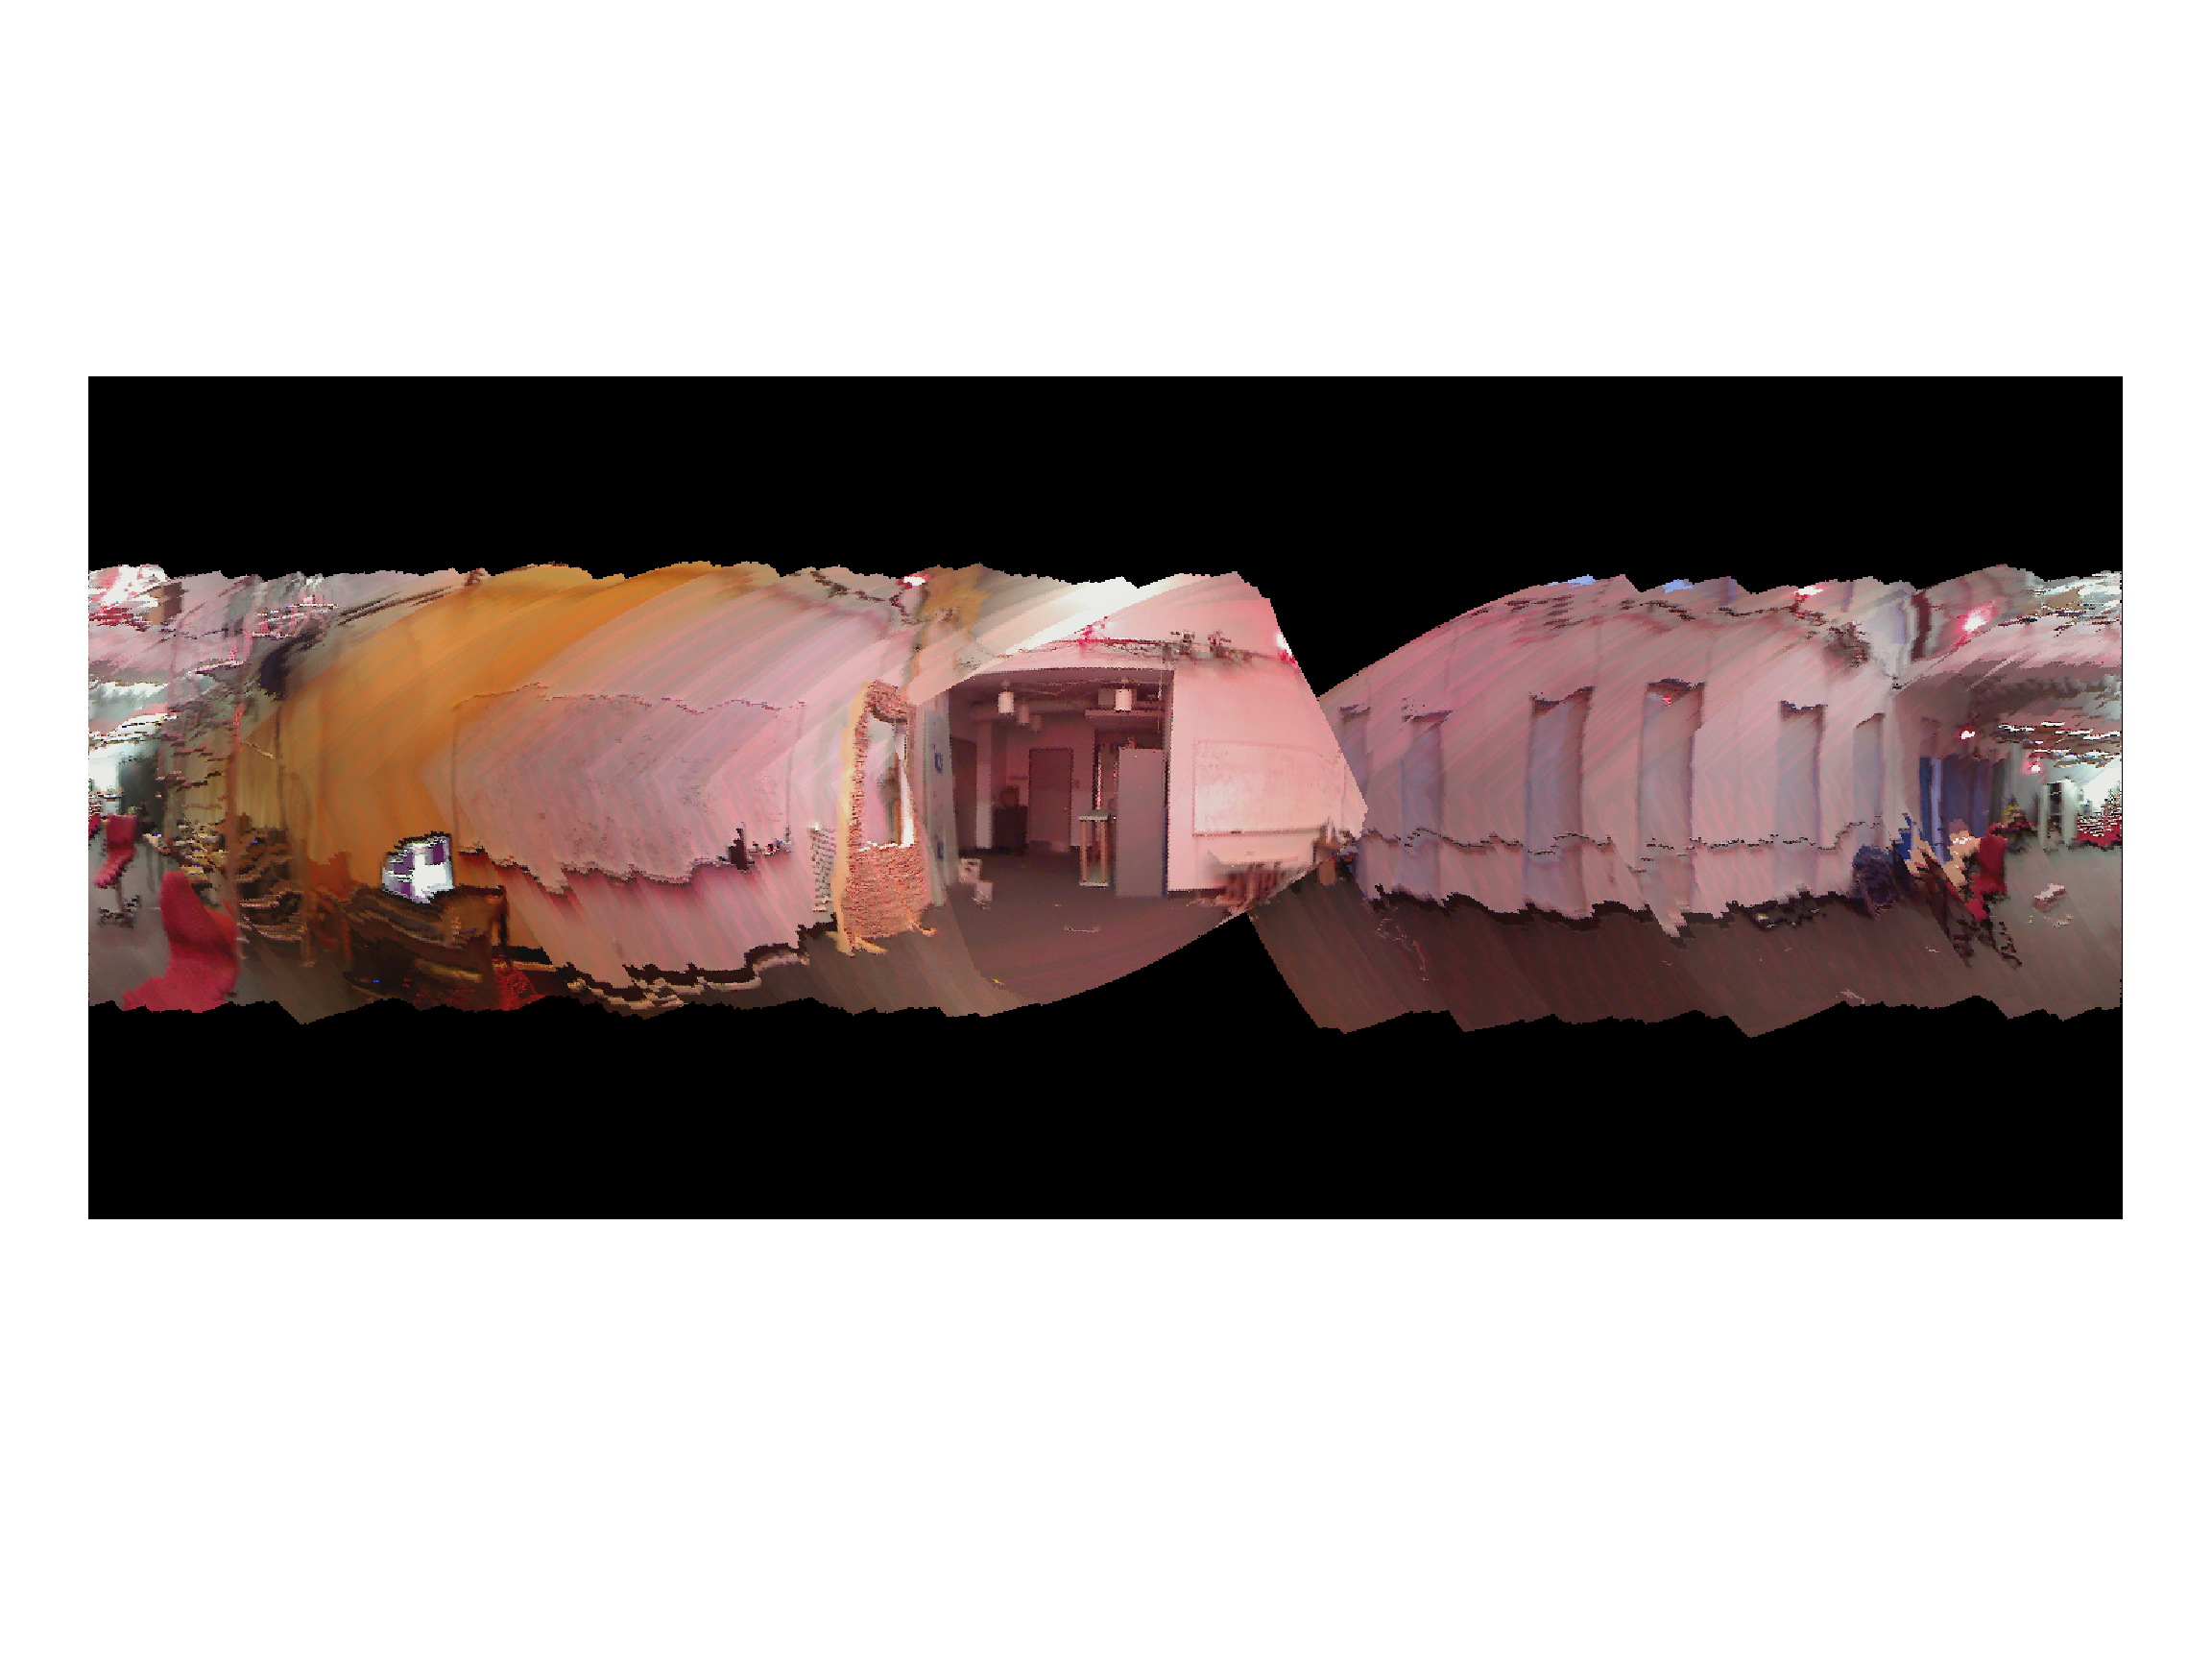
\includegraphics[scale=0.5]{images/pano_test.png} 
\caption{Panoramic image on test set}
\label{fig:pano_test}
\end{figure}


\begin{thebibliography}{2} % Bibliography - this is intentionally simple in this template

\bibitem{Kraft03}
Edgar Kraft, \emph{A quaternion-based unscented kalman filter for orientation tracking}. Information Fusion, 2003. Proceedings of the Sixth International Conference on Information Fusion, Vol. 1 (2003), pp. 47-54. 

\bibitem{Rotations}
\emph{Yaw, pitch, and roll rotations}, http://planning.cs.uiuc.edu/node103.html

\bibitem{3dtrans}
\emph{3D Transformations}, http://planning.cs.uiuc.edu/node100.html

\bibitem{UKF97}
Julier, Simon J., and Jeffrey K. Uhlmann. \emph{New extension of the Kalman filter to nonlinear systems.} AeroSense'97. International Society for Optics and Photonics, 1997.

\end{thebibliography}


\end{document}